% !TEX root = ../Coherence.tex


%%%%%%%%%%%%%%%%%%%%%%%%%%%%%%%%%%%%%

\subsection{Symmetric monoidal categories} 

\correction{
We now formulate and prove Mac Lane's coherence theorem for \emph{symmetric} monoidal categories in the same style as above.  Recall that in a symmetric monoidal category $\mathcal{C}$, in addition to the natural isomorphisms $\beta$, with components $\beta_{\kappa,\mu,\nu}:(\kappa\otimes\mu)\otimes\nu\to
\kappa\otimes(\mu\otimes\nu)$, there are involutive natural transformations $\tau$, with components $\tau_{\mu,\nu}:\mu\otimes\nu\to\nu\otimes\mu$.
Here, we use $\kappa,\mu,\nu,\ldots$ to range over the objects of the category, consistently with the notation used in~\cref{ss:def-catoperads,ss:coherence-catoperads}.
In addition to the pentagons, obtained from the first pentagon in~\cref{def:catoperad} by replacing $\circ$ with $\otimes$, there are hexagons 
\begin{center}
\resizebox{0.4\linewidth}{!}{
    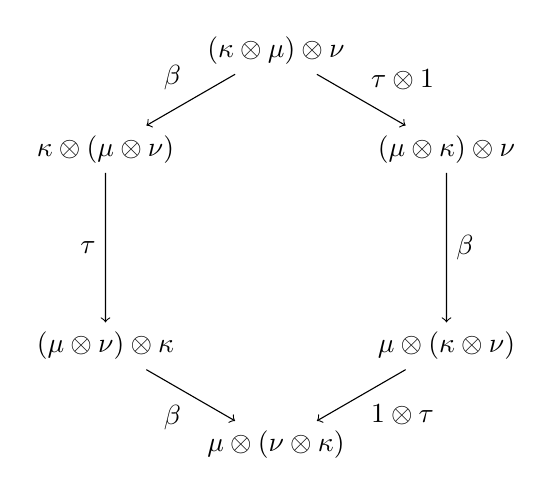
\begin{tikzpicture}[scale=2.5]
    \node (P1) at (0,1) {$(\kappa\otimes \mu) \otimes \nu$};
    \node (P2) at (-0.866,0.5) {$\kappa\otimes (\mu \otimes \nu)$};
    \node (P3) at (-0.866,-0.5) {$(\mu \otimes \nu) \otimes \kappa$};
    \node (P4) at (0,-1) {$\mu \otimes (\nu \otimes \kappa)$};
    \node (P5) at (0.866,0.5) {$(\mu \otimes \kappa) \otimes \nu$} ;
    \node (P6) at (0.866,-0.5) {$\mu \otimes (\kappa \otimes \nu)$};
    \draw[->] (P1)--(P2) node[midway,above left] {$\beta$};
    \draw[->] (P2)--(P3) node[midway,left] {$\tau$};
    \draw[->] (P3)--(P4) node[midway,below left] {$\beta$};
    \draw[->] (P1)--(P5) node[midway,above right] {$\tau\otimes 1$};
    \draw[->] (P5)--(P6) node[midway,right] {$\beta$};
    \draw[->] (P6)--(P4) node[midway,below right] {$1\otimes\tau$};
\end{tikzpicture}}
\end{center}
for all objects $\kappa,\mu,\nu$ in $\mathcal{C}$.}

\correction{
In order to state the coherence theorem, we construct a free category on a set $S$ of \defn{generating objects}. 
We define a small category $\mathcal{S}^{\mathrm{ML}}$ whose set of objects $${\cal T}_S=\bigcup\setc{{\cal T}_A}{A \;\mbox{is a non-empty finite subset of}\;S}$$ is defined as follows:
\begin{enumerate}
    \item if $a \in S$, then $a\in{\cal T}_{\set{a}}$;
    \item if $t_1 \in {\cal T}_A$ and $t_2 \in {\cal T}_B$, and if $A\cap B=\emptyset$,  then $t_1 \otimes t_2\in{\cal T}_{A\cup B}$.
\end{enumerate}
We can see the objects of $\mathcal{S}^{\mathrm{ML}}$ as fully parenthesized words over $S$ where letters are not repeated.
We then define a set $M^{\mathrm{ML}}$ of \defn{basic morphisms} $\beta: (t_1 \otimes t_2) \otimes t_3 \leftrightarrow t_1 \otimes (t_2\otimes t_3) : \beta^{-1}$  and $\tau: t_1\otimes t_2 \leftrightarrow t_2 \otimes t_1 : \tau^{-1}$,  for every $t_1,t_2,t_3  \in {\cal T}_S$.
We then define the \defn{generating morphisms} of $\mathcal{S}^{\mathrm{ML}}$ by the following rules:
\begin{enumerate}
    \item if $\phi \in M^{\mathrm{ML}}$, then $\phi$ is a generating morphism; 
    \item if $\phi : t_1 \to t_2$ is a generating morphism and $t_3 \in {\cal T}_S$, then $\phi \otimes \id : t_1 \otimes t_3 \to t_2 \otimes t_3$ and $\id \otimes \phi : t_3 \otimes t_1 \to t_3 \otimes t_2$ are generating morphisms.
\end{enumerate}
We then define $\mathcal{S}^{\mathrm{ML}}$ as the free category over all generating morphisms. 
This finishes the construction of the category $\mathcal{S}^{\mathrm{ML}}$.
\begin{definition}
    We denote by $\mathcal{F}(S)$ the quotient of $\mathcal{S}^{\mathrm{ML}}$ by localization (inverting the $\beta$ morphisms), by the axioms $\tau_{t_1,t_2}\circ \tau_{t_2,t_1}=1$, by the axioms of bifunctors, by the naturality conditions for $\beta$ and $\tau$, and by the coherence conditions of symmetric monoidal categories.
\end{definition}
By freeness, we have that for any symmetric monoidal category $\mathcal{C}$, and for any function $\rho : S \to \obj(\mathcal{C})$, there is a unique functor  $\extd{-}{\mathrm{ML}}:\mathcal{S}^{\mathrm{ML}} \to \mathcal{C}$ which extends $\rho$ and sends the formal basic morphisms to the actual canonical morphisms of $\mathcal{C}$.
This functor factorizes  through the quotient map $[-]^{\mathrm{ML}} :\mathcal{S}^{\mathrm{ML}} \to \mathcal{F}(S)$.}

\correction{
It turns out that Kapranov's topological proof is not based on the above presentation of~$\mathcal{F}(S)$, but on another presentation of this category, that is made explicit in~\cite[Sec.~2]{baralicSimplePermutoassociahedron2019}. 
Let us recall this presentation. 
We define another category $\mathcal{S}^{\mathrm{K}}$ as follows. Its objects are the same as those of $\mathcal{S}^{\mathrm{ML}}$. We define a set $M^{\mathrm{K}}$ of \defn{basic morphisms} $\beta: (t_1 \otimes t_2) \otimes t_3 \leftrightarrow t_1 \otimes (t_2\otimes t_3) : \beta^{-1}$ for every $t_1,t_2,t_3  \in {\cal T}_S$, and $\tau: a\otimes b \leftrightarrow b \otimes a : \tau^{-1}$ for every $a,b \in S$, i.e., we \emph{limit $\tau$ to generating objects}.
\defn{Generating morphisms} are defined in the same way as for $\mathcal{S}^{\mathrm{ML}}$.
We note that by construction $\mathcal{S}^{\mathrm{K}}$ is a wide subcategory of $\mathcal{S}^{\mathrm{ML}}$.
\begin{definition}
    \label{def:free-Kap}
    We denote  by $\mathcal{F}(S)^{\mathrm{K}}$ the quotient of $\mathcal{S}^{\mathrm{K}}$ by localization (inverting the $\beta$ morphisms), by the axioms $\tau_{a,b}\circ \tau_{b,a}=1$, by the axioms of bifunctors, by the naturality conditions for $\beta$, by the coherence conditions of  monoidal categories, and by the axioms in dodecagonal form given by the solid arrows in~\cref{fig:dodecagon} (left), for $a,b,c$ ranging over $S$ only.
\end{definition}
\begin{figure}[h!]
\begin{center}
\resizebox{\linewidth}{!}{
 \begin{tikzpicture}[scale=6.5]
    \node (P1) at (0,1) {$(a \otimes b) \otimes c$};
    \node (P2) at (-0.5,0.866) {$a \otimes (b \otimes c)$};
    \node (P3) at (-0.866,0.5) {$a \otimes (c \otimes b)$};
    \node (P4) at (-1,0) {$(a \otimes c) \otimes b$};
    \node (P5) at (-0.866,-0.5) {$(c \otimes a) \otimes b$} ;
    \node (P6) at (-0.5,-0.866) {$c \otimes (a \otimes b)$};
    \node (P7) at (0,-1) {$c \otimes (b \otimes a)$};
    \node (P8) at (0.5,-0.866) {$(c \otimes b) \otimes a$};
    \node (P9) at (0.866,-0.5) {$(b \otimes c) \otimes a$};
    \node (P10) at (1,0) {$b \otimes (c \otimes a)$};
    \node (P11) at (0.866,0.5) {$b \otimes (a \otimes c)$} ;
    \node (P12) at (0.5,0.866) {$(b \otimes a) \otimes c$};
    \draw[->] (P1)--(P2) node[midway,above left] {$\beta$};
    \draw[->] (P2)--(P3) node[midway,above left] {$1\otimes\tau$};
    \draw[->] (P3)--(P4) node[midway,above left] {$\beta^{-1}$};
    \draw[->] (P4)--(P5) node[midway,below left] {$\tau\otimes 1$};
    \draw[->] (P5)--(P6) node[midway,below left] {$\beta$};
    \draw[->] (P6)--(P7) node[midway,below left] {$1\otimes\tau$};
    \draw[->] (P1)--(P12) node[midway,above right] {$\tau\otimes 1$};
    \draw[->] (P12)--(P11) node[midway,above right] {$\beta$};
    \draw[->] (P11)--(P10) node[midway,above right] {$1\otimes\tau$};
    \draw[->] (P10)--(P9) node[midway,below right] {$\beta^{-1}$};
    \draw[->] (P9)--(P8) node[midway,below right] {$\tau\otimes 1$};
    \draw[->] (P8)--(P7) node[midway,below right] {$\beta$};
    \draw[->,dashed] (P2)--(P9) node[midway,above right] {$\tau$};
    \draw[->,dashed] (P3)--(P8) node[midway,below left] {$\tau$};
\end{tikzpicture}
\quad\quad
 \begin{tikzpicture}[scale=6.5]
    \node (P1) at (0,1) {$(\set{a}  \set{b})  \set{c}$};
    \node (P2) at (-0.5,0.866) {$\set{a}  (\set{b}  \set{c})$};
    \node (P3) at (-0.866,0.5) {$\set{a}  (\set{c}  \set{b})$};
    \node (P4) at (-1,0) {$(\set{a}  \set{c})  \set{b}$};
    \node (P5) at (-0.866,-0.5) {$(\set{c}  \set{a})  \set{b}$} ;
    \node (P6) at (-0.5,-0.866) {$\set{c}  (\set{a}  \set{b})$};
    \node (P7) at (0,-1) {$\set{c}  (\set{b}  \set{a})$};
    \node (P8) at (0.5,-0.866) {$(\set{c}  \set{b})  \set{a}$};
    \node (P9) at (0.866,-0.5) {$(\set{b}  \set{c})  \set{a}$};
    \node (P10) at (1,0) {$\set{b}  (\set{c}  \set{a})$};
    \node (P11) at (0.866,0.5) {$\set{b}  (\set{a}  \set{c})$} ;
    \node (P12) at (0.5,0.866) {$(\set{b}  \set{a})  \set{c}$};
    \node (P13) at (0,0) {$\set{a,b,c}$} ;
    \draw[-] (P1)--(P2) node[midway,above left] {$\set{a}\set{b}\set{c}$};
    \draw[-] (P2)--(P3) node[midway,above left] {$\set{a}\set{b,c}$};
    \draw[-] (P3)--(P4) node[midway,above left] {$\set{a}\set{c}\set{b}$};
    \draw[-] (P4)--(P5) node[midway,below left] {$\set{a,c}\set{b}$};
    \draw[-] (P5)--(P6) node[midway,below left] {$\set{c}\set{a}\set{b}$};
    \draw[-] (P6)--(P7) node[midway,below left] {$\set{c}\set{a,b}$};
    \draw[-] (P1)--(P12) node[midway,above right] {$\set{a,b}\set{c}$};
    \draw[-] (P12)--(P11) node[midway,above right] {$\set{b}\set{a}\set{c}$};
    \draw[-] (P11)--(P10) node[midway,above right] {$\set{b}\set{a,c}$};
    \draw[-] (P10)--(P9) node[midway,below right] {$\set{b}\set{c}\set{a}$};
    \draw[-] (P9)--(P8) node[midway,below right] {$\set{b,c}\set{a}$};
    \draw[-] (P8)--(P7) node[midway,below right] {$\set{c}\set{b}\set{a}$};
\end{tikzpicture}} 
\end{center}
\caption{Kapranov dodecagons.}
\label{fig:dodecagon}
\end{figure}}

\correction{
We pause here to reflect on the difference between the two presentations. In the second one, we have less generators, and we have lost hexagons. For an intuition, here is how Mac Lane himself motivated his hexagonal axioms (verbatim, just changing the notation to fit with ours) in~\cite{MacLane63}:
\begin{quote}
    \label{q:ML}
The instance $\tau_{\kappa\otimes \mu,\nu}$ interchanges the block $\kappa\mu$ with the single letter $\nu$; the hexagon condition states that this interchange may be replaced by two instances of $\tau$ which interchange single letters with $\nu$. Repeated such replacement using instances of the hexagon shows that any interchange of successive blocks may be replaced by interchanges of successive letters.
\end{quote}
In other words, hexagons are now taken as definitions rather than axioms. But how do we guarantee that the  general $\tau$ morphisms defined in this way define a natural transformation? This is what the dodecagons are for.}

\correction{
Let $\mathcal{C}$  be a symmetric monoidal category. 
By freeness, any function $\rho : S \to \obj(\mathcal{C})$ extends uniquely to a functor $\extd{-}{\mathrm{K}}:\mathcal{S}^{\mathrm{K}} \to \mathcal{C}$.
This functor is the restriction of $\extd{-}{\mathrm{ML}}$ to $\mathcal{S}^{\mathrm{K}}$, and factorizes through the quotient functor $[-]^{\mathrm{K}}:\mathcal{S}^{\mathrm{K}}\to  \mathcal{F}(S)^{\mathrm{K}}$.
\begin{thm}[Kapranov coherence theorem for symmetric monoidal categories]
\label{thm:coherence-Kapranov}
 For any two parallel morphisms $\phi_1,\phi_2: t_1 \to t_2$ in~$\mathcal{S}^{\mathrm{K}}$, we have~$[\phi_1]^{\mathrm{K}}=[\phi_2]^{\mathrm{K}}$.
\end{thm}}

\correction{
In order to prove this ``Kapranov style'' coherence, we need to first recall the construction of the \defn{permuto-associahedra}, a family of polytopes whose faces are in bijection with parenthesized ordered partitions of a finite set.
We refer to \cite[Sec.~9.3]{Ziegler95} for details, see also \cite{kapranov1993} and \cite{reinerCoxeterassociahedra1994}.
Given a finite set $A$ of cardinal $n$ and a parenthesized permutation $\sigma$ of its elements, one associates a section $\gamma^\sigma$ of the projection from the $n$-cube to the cyclic polygon with $n+1$ vertices \cite[Ex.~9.14]{Ziegler95}, whose integral over the base gives a point~$M(\sigma)$ in $\R^n$. 
The \defn{permuto-associahedron} $P_A$ is the convex hull of the points $M(\sigma)$, for all parenthesized permutations $\sigma$ of the elements of $A$. 
It has dimension $n-1$. 
One then shows that the poset of parenthesized ordered partitions of $A$, ordered according to the rules below, is isomorphic to the poset of faces of $P_A$ \cite[Thm.~9.15]{Ziegler95}.}

\correction{Parenthesized ordered partitions of $A$ can be drawn as planar trees whose leaves are decorated with the parts of a partition of $A$.
The subface relation $\prec$ is defined by two clauses: one can contract an edge of the tree, or remove a node all of whose  incoming edges are leaves and decorate its outcoming edge -- now a leaf -- with the union of the decorations of those incoming edges.
The maximal face is $A$.
For example, with $A=\set{a_1,\ldots,a_7}$, the following is a face:
$$\begin{array}{l}
(\set{a_1} \set{a_4} \set{a_2,a_6}) \set{a_3,a_5,a_7}
\end{array}$$
which is covered by the following two elements.
$$\begin{array}{lll}
(\set{a_1} \set{a_4} \set{a_2,a_6}) \set{a_3,a_5,a_7} & \prec & \set{a_1} \set{a_4} \set{a_2,a_6} \set{a_3,a_5,a_7} \\
(\set{a_1} \set{a_4} \set{a_2,a_6}) \set{a_3,a_5,a_7} & \prec &  \set{a_1,a_2,a_4,a_6} \set{a_3,a_5,a_7}.
\end{array}$$}

\correction{Given the set $S$, let us consider the collection $\mathcal{P}(S)$ of polytopes with one copy of the permuto-associahedron $P_A$ for each finite subset $A \subset S$.
\begin{proposition}
    There are bijections between
\begin{enumerate}
    \item objects of $\mathcal{S}^{\mathrm{K}}$ and vertices of the permuto-associahedra in $\mathcal{P}(S)$,
    \item generating morphisms of $\mathcal{S}^{\mathrm{K}}$ and edges of the permuto-associahedra in $\mathcal{P}(S)$,
    \item bifunctoriality, naturality and coherence diagrams and $2$-faces of the permuto-associahedra in $\mathcal{P}(S)$.
\end{enumerate}
\end{proposition}
\begin{proof}
    The 0-dimensional faces of $P_A$ are fully parenthesized words whose letters are singletons, and are in obvious bijective correspondence with the elements of ${\cal T}_A$. 
The 1-dimensional faces are 
\begin{itemize}
\item
either fully parenthesized words whose letters are singletons but for one letter which is a two-element set $\set{a_i,a_j}$ and feature an application of the basic morphism $\tau_{a_i,a_j}$, 
\item or an ``almost'' fully parenthesized word of singletons, with just one parenthesis removed, yielding a subword $(\set{a_i} \set{a_j} \set{a_k})$, featuring an application of the basic morphism $\beta_{a_i,a_j,a_k}$ or $\beta_{a_i,a_j,a_k}^{-1}$
-- the orientation of the edge being ``decided'' by the shape of its end vertices.
\end{itemize}
Finally, the 2-dimensional faces can be analyzed much in the same way as in~\cref{prop:bijection-nestings}, and seen to correspond to bifunctoriality, naturality of $\beta$, and to the pentagons and dodecagons. 
We have pictured the poset view of the 
latter in~\cref{fig:dodecagon} (right). 
The reader can also convince himself on this figure how the orientation of the $\beta$ arrows on the left can be reconstructed from the non oriented dodecagon on the right.
\end{proof}
\begin{proof}[Proof of \cref{thm:coherence-Kapranov}]
The proof is similar to the proof of \cref{thm:coherence-operahedra}, using either the Van Kampen (\cref{thm:top-coherence}) or Morse (\cref{prop:polytopes,p:second-proof}) technique.
\end{proof}
\begin{rem}
    Note that contrary to the case of operahedra, there does not seem to exist a generic vector inducing an orientation of the edges of the permuto-associahedra which coincides with the orientation of the $\beta$ and $\tau$ arrows, as the dodecagon (\cref{fig:dodecagon}, left) involves $\beta^{-1}$ arrows. 
\end{rem}
\begin{rem}
    Notice that the permuto-associahedra are not simple polytopes.
    Alternatively, one could use the same strategy with the \emph{simple permuto-associahedra} from~\cite{baralicSimplePermutoassociahedron2019}, involving yet another presentation of symmetric monoidal categories.
\end{rem}
The following proposition establishes relations between the Mac Lane and Kapranov presentations of symmetric monoidal categories.
\begin{proposition}[Kapranov--Mac Lane comparison]
\label{Kapranov-MacLane}
\leavevmode
\begin{enumerate}
\item Let $\phi_1,\phi_2: t_1 \to t_2$  be parallel morphisms of $\mathcal{S}^{\mathrm{K}}$, and suppose that $[\phi_1]^{\mathrm{K}}=[\phi_2]^{\mathrm{K}}$. Then $[\phi_1]^{\mathrm{ML}}=[\phi_2]^{\mathrm{ML}}$.
\item Let $\phi$ be a morphism of $\mathcal{S}^{\mathrm{ML}}$. Then there is a morphism $\psi$ of 
$\mathcal{S}^{\mathrm{K}}$ such that $[\phi]^{\mathrm{ML}}=[\psi]^{\mathrm{ML}}$.
\end{enumerate}
\end{proposition}
\begin{proof}
The proof of Point (1) is visualized in~\cref{fig:dodecagon} (left).  
The two dotted lines delimit two Mac Lane hexagons on the top and at the bottom and a naturality square in the middle.
Explicitly, the two dotted $\tau$-morphisms are $\tau_{a,b\otimes c}$ and $\tau_{a,c\otimes b}$.  
As for Point (2), we observe that a morphism $\psi$ as in the statement can be obtained by repeatedly applying the procedure described by Mac Lane in the quotation which follows \cref{def:free-Kap} above.
\end{proof}
\begin{thm}[Mac Lane coherence theorem for symmetric monoidal categories]
\label{thm:coherence-MacLane}
    For any symmetric monoidal category $\mathcal{C}$, for any  function $\rho : S \to \obj(\mathcal{C})$, and for any two parallel morphisms $\phi_1,\phi_2: t_1 \to t_2$ in~$\mathcal{S}^{\mathrm{ML}}$, we have $\extd{\phi_1}{\mathrm{ML}}=\extd{\phi_2}{\mathrm{ML}}$.
\end{thm}
\begin{proof} 
Since the functor $\extd{-}{\mathrm{ML}}$ factorizes through the functor $[-]^{\mathrm{ML}}$, it is enough to prove that $[\phi_1]^{\mathrm{ML}}=
[\phi_2]^{\mathrm{ML}}$. 
By Point (2) of~\cref{Kapranov-MacLane}, there exist $\psi_1$ and $\psi_2$ in $\mathcal{S}^{\mathrm{K}}$ such that $[\psi_1]^{\mathrm{ML}}=[\phi_1]^{\mathrm{ML}}$ and 
$[\psi_2]^{\mathrm{ML}}=[\phi_2]^{\mathrm{ML}}$.
In particular $\psi_1$ and $\psi_2$ are parallel, so by~\cref{thm:coherence-Kapranov} we get $[\psi_1]^{\mathrm{K}}=[\psi_2]^{\mathrm{K}}$, and by Point (1) of~\cref{Kapranov-MacLane} we have $[\psi_1]^{\mathrm{ML}}=[\psi_2]^{\mathrm{ML}}$.
Thus, we have $[\phi_1]^{\mathrm{ML}} = [\psi_1]^{\mathrm{ML}} =  [\psi_2]^{\mathrm{ML}} =  [\phi_2]^{\mathrm{ML}}$, which concludes the proof.
\end{proof}
\begin{rem}
One can see easily that this proof  also shows that the categories  $\mathcal{F}(S)^{\mathrm{K}}$ and~$\mathcal{F}(S)$ are isomorphic.  
The statement of this fact is unrelated to coherence issues, but  its proof relies on Kapranov style coherence.
\end{rem}}
